\begin{figure}[b!]
    \centering
    \begin{tabular}[l]{cc}
    \begin{subfigure}{0.49\textwidth}
        \centering
        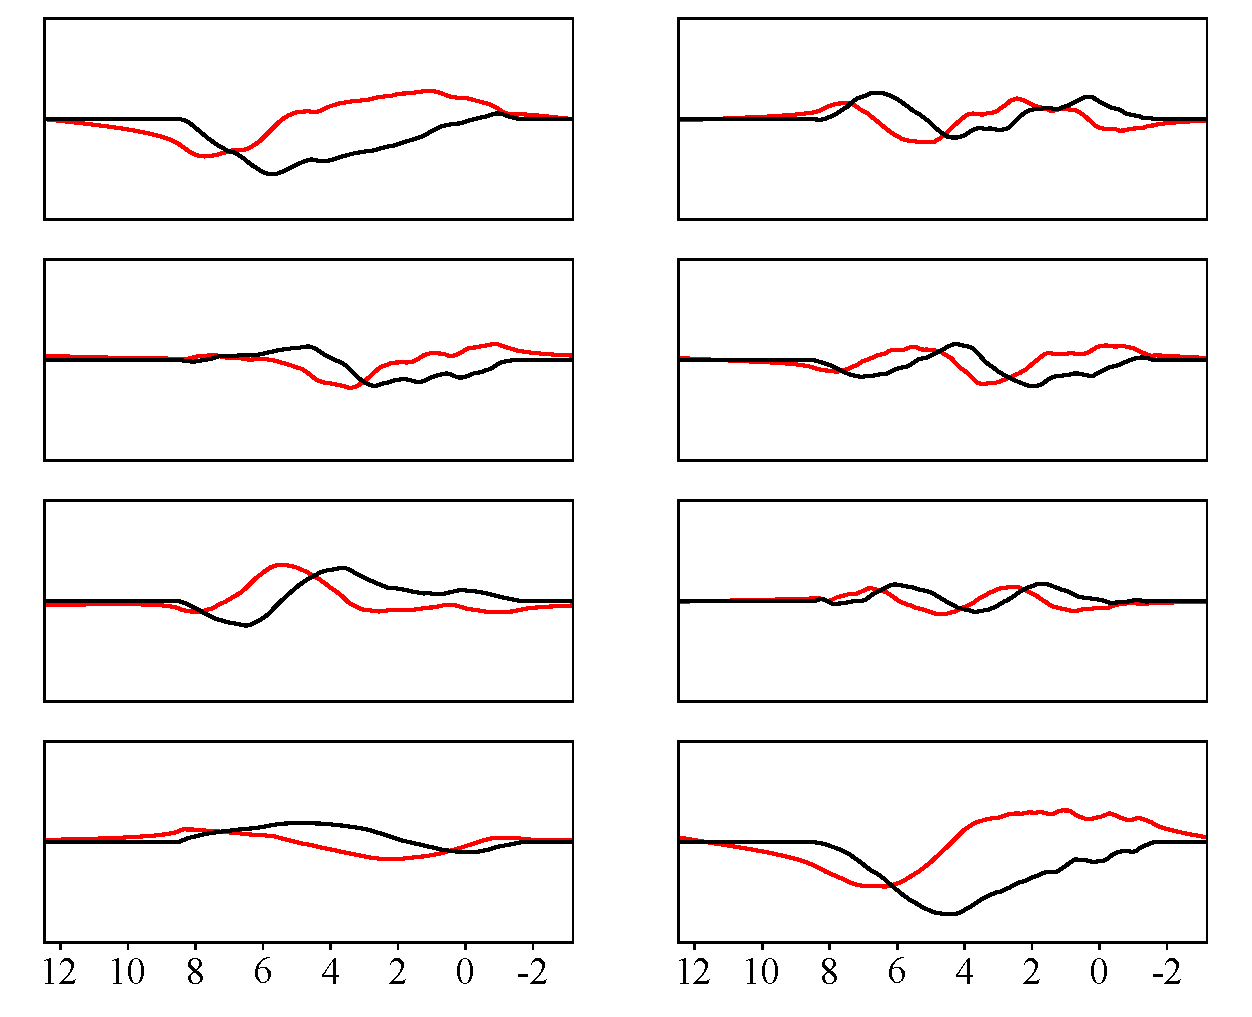
\includegraphics[width=0.95\textwidth,keepaspectratio]{images/random_walks/baseline_walks_edited.eps}
        \caption{Simulated baselines}
        \label{fig:baseline_region}
    \end{subfigure} &
    
    \begin{subfigure}{0.49\textwidth}
        \centering
        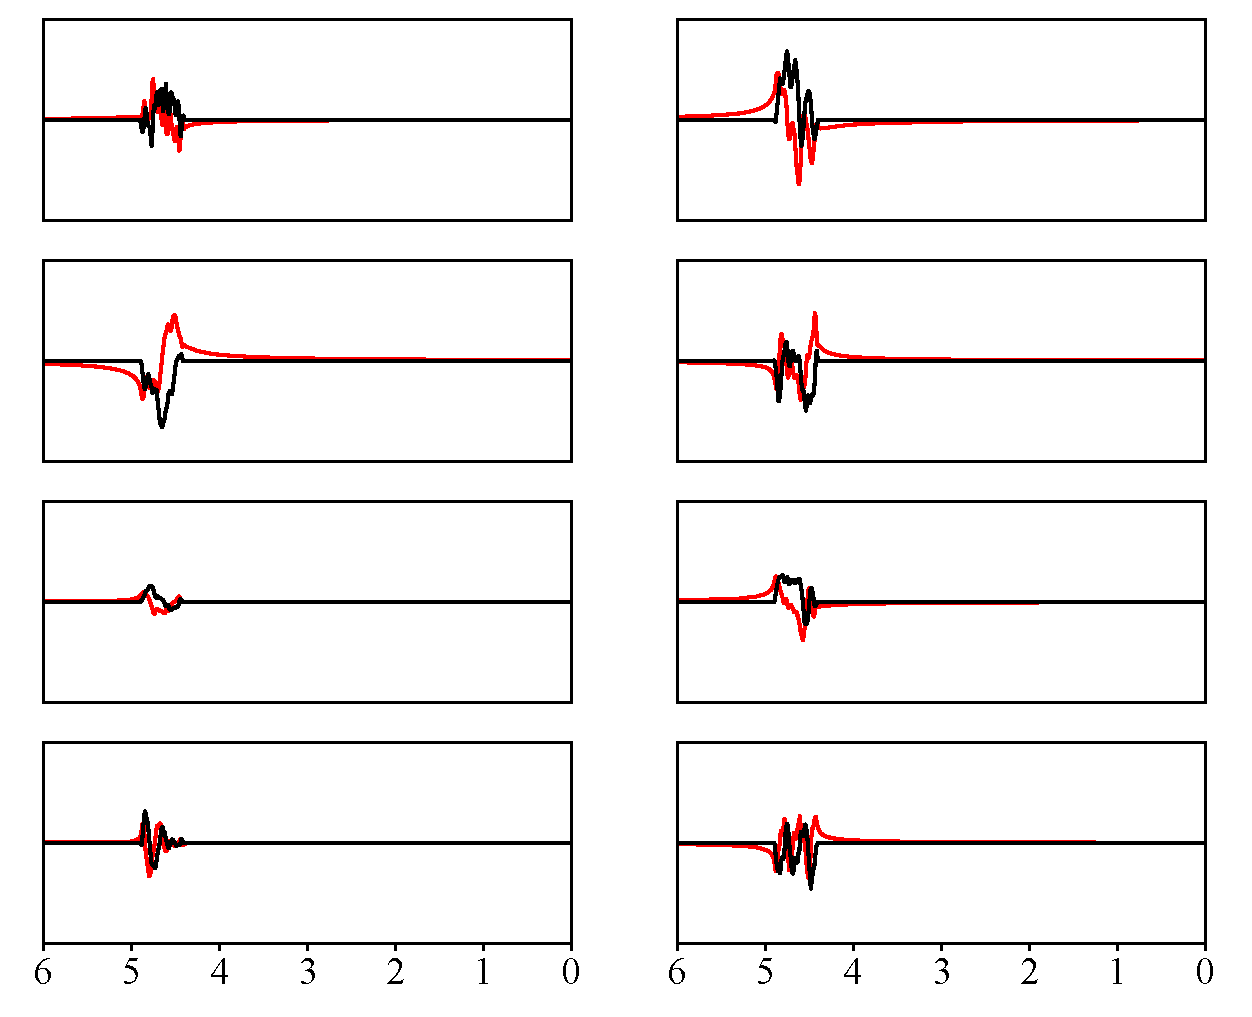
\includegraphics[width=0.95\textwidth,keepaspectratio]{images/random_walks/reswater_walks_edited.eps}
        \caption{Simulated residual water}
        \label{fig:reswater_region}
    \end{subfigure}
    \end{tabular}
    \caption{Simulated  samples of spectral baselines and residual water regions using the pseudo-random bounded walk generator. The blue lines are the raw simulations. The red lines are the smoothed versions that are then returned and applied to the simulated spectra.}
    \label{fig:random walk generator}
\end{figure}
